\documentclass{report}
\usepackage[utf8]{inputenc}
\usepackage[margin=20mm]{geometry}
\usepackage{graphicx}
\graphicspath{ {./img/} }
\usepackage{amsmath}
\usepackage{tabularx}
\usepackage{subcaption}
\usepackage{float}
\usepackage{titlesec}
\usepackage{enumitem}
\usepackage{amsthm}
\renewcommand*\contentsname{Indice}

% El psy kongroo
% Definizione di un ambiente per i teoremi
\newtheorem{teorema}{Teorema}
\newtheorem{definizione}{Definizione}

% Definire lo stile per le sezioni e sottosezioni
\titleformat{\section}[block]
  {\normalfont\fontsize{20}{24}\bfseries\filcenter} % Font size and style
  {\thesection}{10pt}{} % Section number format

\titleformat{\subsection}[block]
  {\normalfont\fontsize{15}{18}\bfseries} % Font size and style
  {\thesubsection}{10pt}{} % Subsection number format

% Rimuovere l'indentazione a sinistra dei titoli delle sezioni e sottosezioni
\titlespacing*{\section}{0pt}{*2}{*1.5}
\titlespacing*{\subsection}{0pt}{*1.5}{*1}


% Gap righe
\renewcommand{\arraystretch}{1.6}


\title{Basi di dati Appunti\\ -\\ secondo parziale}
\author{Dimitri}
\date{A.A. 2024/2025}

\begin{document}
\maketitle
\newpage
\tableofcontents
\newpage
%sezione non completa

\chapter{Algebra Relazionale}
\section{Introduzione}
L'algebra relazionale è un linguaggio procedurale formale di tipo algebrico i cui operandi sono relazioni.
Questo linguaggio non è usato nelle implementazioni dei vari DBMS ma definisce in maniera semplice tutte le operazioni tipiche dei diversi linguaggi di interrogazione.
Da un punto di vista didattico l’algebra relazionale è utile perché essendo svincolata dai “dettagli
implementativi” dell’SQL (o di altri linguaggi), permette di comprendere rapidamente la tecnica d’uso dei linguaggi di interrogazione per basi di dati relazionali.\\
\section{Operatori}
\subsection{Introduzione}
In Algebra relazionale è possibile classificare i diversi operatori in base alla derivabilità oppure in modo funzionale. Questi operatori possono essere binari o unari, e tramite questi ultimi vengono descritte le procedure di interrogazione.\\
Nella classificazione in base alla derivabilità si distiguono 6 operatori di base e diversi derivati:\\
\textbf{Operatori di Base:}
\begin{itemize}
    \item Selezione
    \item Proiezione
    \item Ridenominazione
    \item Unione
    \item Differenza
    \item Prodotto cartesiano
\end{itemize}
\textbf{Operatori derivati:}
\begin{itemize}
    \item Intersezione
    \item Join
\end{itemize}
\newpage
\subsection{Selezione $\sigma$}
La selezione è un'operazione unaria. Seleziona le tuple di una relazione che soddisfano un predicato producendo un sottoinsieme delle stesse, (ossia seleziona le righe della tabella che rispettano la condizione data, ricordiamo che con tuple si intendono le righe della tabella mentre con attributi le singole colonne).\\
Lo schema della relazione risultato è lo stesso di quella di origine ed il predicato è costituito dal nome di un attributo, da un operatore, e da un altro argomento che può essere un attributo o un valore
costante.\\
$$\sigma_{\text{predicato}}(relazione)$$\\
La cardinalità di questa operazione è la seguente:\\
$$ 0 \leq |\sigma_{\text{F}}(R)| \leq |R|$$\\

\subsection{Proiezione $\Pi$}
La proiezione è un'operazione unaria. Data una relazione, la sua proiezione su un dato insieme di attributi è costituita dalla tabella generata dagli attributi specificati, contenente tutte le tuple della tabella di partenza, (ossia estrae tutte le colonne corrispondenti alla lista di attributi specificati).\\
$$\Pi_{\text{lista attributi}}(relazione)$$\\
La cardinalità di questa operazione è la seguente:\\
$$min(|R|, 1) \leq \Pi_{\text{y}}(R) \leq |R|$$\\

\subsection{Ridenominazione $\rho$}
A volte in preparazione all’esecuzione di una interrogazione o in seguito ad una sua esecuzione si ha bisogno di rinominare gli attributi di una relazione. A tal fine l’operatore di ridenominazione che permette di ottenere una nuova tabella con i nuovi nomi per gli attributi modificati e che ha le stesse tuple della tabella originale.\\
$$\rho_{\text{vecchio nome $\to$ nuovo nome}}(relazione)$$\\

\subsection{Unione $\cup$}
L’unione fra due tabelle è rappresentata da una tabella costituita dall’unione “matematica” delle due tabelle, dove quindi sono presenti le tuple della prima tabella e quelle della seconda. Affinché l’unione abbia senso, è necessario che:
\begin{itemize}
    \item le due tabelle abbiano lo stesso numero di attributi;
    \item i tipi degli attributi corrispondenti siano uguali;
\end{itemize}
Se il numero degli attributi delle due relazioni (tabelle) non è uguale, si genera un errore.\\
La cardinalità di questa operazione è la seguente:\\
$$max(|R1|, |R2|) \leq |R1 \cup R2| \leq |R1| + |R2|$$\\

\subsection{Differenza -}
La differenza fra due tabelle A e B è una tabella che contiene le tuple che sono presenti in A ma non in
B. Come nel caso dedll'unione, questa operazione può essere eseguita solo se le relazioni hanno lo stesso grado (numero di colonne) e gli attributi sono compatibili.\\
La cardinalità di questa operazione è la seguente:\\
$$0 \leq |R1 - R2| \leq |R1|$$\\

\subsection{Prodotto Cartesiano $\times$}
Il prodotto cartesiano fra due tabelle è una tabella con schema la somma degli schemi, se due attributi
sono uguali questi sono ripetuti le tuple della tabella sono il risultato del prodotto cartesiano dei suoi elementi, ossia da tutte le coppie possibili composte dagli elementi appartenenti alle due relazioni.\\
$$R1\times R2$$\\
La cardinalità di questa operazione è la seguente (ricordiamo che se il Join è completo il limite inferiore diventa $max(|R1|,|R2|)$):\\
$$|R1 \times R2| = |R1| \cdot |R2|$$\\

\subsection{Intersezione $\cap$}
Il risultato dell'operazione di intersezione tra due relazioni è una relazione contenente le tuple che appartengono ad entrambe le relazioni, anche in questo caso valgono le stesse condizioni di unione e differenza per la validità dell'operazione.\\
$$R1 \cap R2$$\\
La cardinalità di questa operazione è la seguente:\\
$$ 0 \leq |R1 \cap R2| \leq min(|R1|, |R2|)$$\\

\section{Join}
\subsection{Introduzione}
E’ l’operatore più caratteristico dell’algebra relazionale, in quanto è quello che permette di correlare dati contenuti in relazioni diverse confrontando i valori comuni contenuti in esse.\\
Esistono diverse varianti di tale operatore comunque riconducibili l’una con l’altra:
\begin{itemize} 
    \item Join Naturale
    \item Join Esterni
    \item Theta Join ed Equi Join\\
\end{itemize}
\subsection{Join Naturale $\bowtie$}
Il Join naturale è un operatore binario che correla dati in relazioni diverse sulla base dei valori uguali in attributi con lo stesso nome. La relazione risultante è una tabella che ha come attributi l’unione degli attributi delle tabelle iniziali e contiene solamente le tuple che hanno valori uguali negli attributi in comune.\\
Quando non si hanno attributi comuni il join naturale diventa un prodotto cartesiano, perch\'e genera tutte le possibili coppie. 

\paragraph{Esempio.}  Prendiamo lo schema: \\

\noindent\texttt{DOCENTE(\underline{CFDocente}, Nome, Cognome) \\
CORSO(\underline{Nome}, CFDocente)}\\

\noindent Si richiede di produrre l'insieme dei corsi riportando: nome del corso e cognome del docente.
\[ \Pi_{\text{NomeCorso, Cognome}}(\rho_{\text{Nome $\to$ NomeCorso}}(CORSO) \bowtie \thickspace DOCENTE)\]
Graficamente si ottiene:

\begin{center}
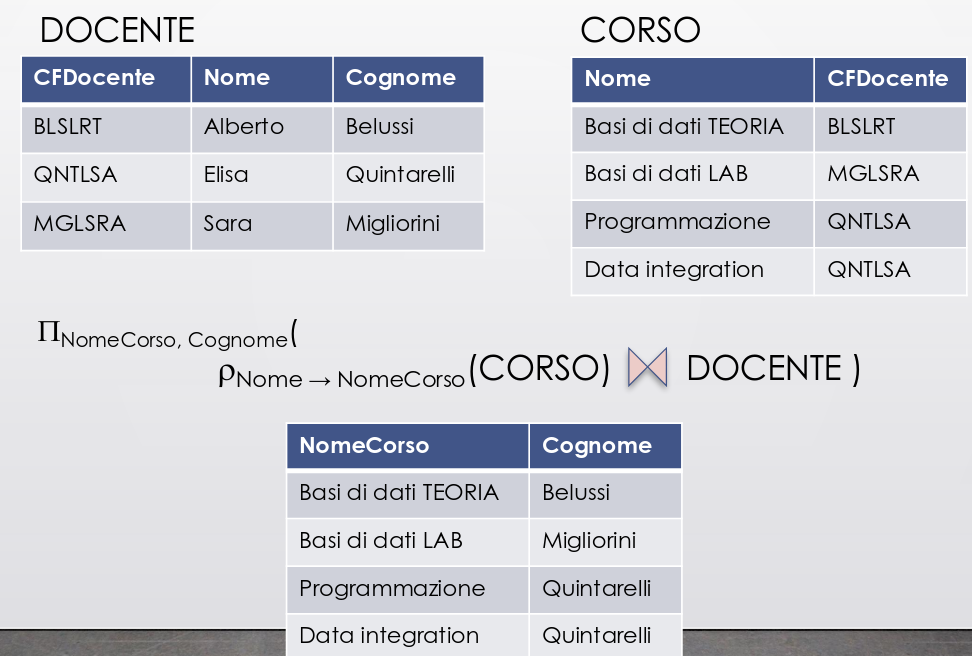
\includegraphics[scale=0.35]{join_example}

\end{center}


Il Join può essere ottenuto tramite un prodotto cartesiano e una selezione imponendo l’uguaglianza su tutti gli attributi in comune:\\
$$\sigma_{\text{NomeCorso = Nome}}(DOCENTE \times CORSO)$$\\
Il Join si dice completo se ogni tupla della relazione A contribuisce a generare almeno una tupla della relazione risultato, altrimenti si dice incompleto e le tuple che non contribuiscono al risultato si chiamano \textbf{dangling tuples}.

La cardinalità del Join Naturale è, in generale:
\[0 \leq |R1 \bowtie R2| \leq |R1| \cdot |R2|\]
Se il join \`e completo la cardinalit\`a diventa:
\[ max(|R1|, |R2|) \leq |R1 \bowtie R2| \leq |R1| \cdot |R2| \]

\newpage
\subsection{Theta Join ed Equi Join}
Nel caso del Theta Join, l'operatore della condizione di selezione eseguita dopo il prodotto cartesiano viene esplicitato. Nel caso in cui OP (ossia l'operatore nella selezione) sia composta solo da uguaglianze, l’operazione prende il nome di Equi-join.\\
$$ A \bowtie_{\text{$\theta$}}B$$\\
Ricordiamo che è possibile riscrivere il Join tramite il prodotto cartesiano e la selezione:\\
$$\sigma_{\text{A.attributo\_comune $\theta$ B.attributo\_comune}}(A \times B)$$\\
Dove $\theta$ è l'operatore.\\
Solitamenta questi due operatori vengono usati più del Natural Join dato che non è obbligatoria l'uguaglianza del nome degli attributi e sono più modellabili.\\

\newpage
\section{Ottimizzazione}
\subsection{Valori NULL}
E’ opportuno estendere l’algebra relazionale affinché possa manipolare anche relazioni che contengono valori nulli (NULL). Le operazioni che devono essere raffinate per gestire relazioni che contengono valori nulli sono in particolare \textbf{selezione} e \textbf{Join Naturale}.\\
Le altre operazioni riportano semplicemente nelle tuple del risultato il valore nullo presente sulle tuple di input.\\\\
Nel caso della \textbf{selezione} abbiamo che $\sigma_\text{A $\theta$ B}$ risulta essere falsa (quindi non selezionare quella determinata tupla) se uno dei due attributi A o B è NULL (anche se messo a confronto con una costante). Nel caso invece ci sia un'operazione atomica del tipo "A is NULL" allora risulterà vera se e solo se A è NULL.\\\\
Anche il \textbf{Join Naturale} si comporta in modo simile, infatti se anche solo uno degli attributi comuni risulta essere NULL allora il Join sarà falso su quella tupla. Si ricorda che "NULL = NULL" è sempre falso.\\

\subsection{Ottimizzatore}
Ogni espressione DML ricevuta dal DBMS viene sottoposta ad un processo di elaborazione, tra cui, anche uno di ottimizzazione. L’ottimizzatore genera un’espressione equivalente all’interrogazione di input e di costo inferiore (il costo viene valutato in termini di dimensione dei risultati intermedi).\\
L’ottimizzatore esegue trasformazioni di equivalenza allo scopo di riddurre la dimensione dei risultati intermedi.\\
Le principali sono quattro e sono le seguenti:
\begin{itemize}
    \item \textbf{Atomizzazione delle selezioni:} una congiunzione di selezioni può essere sostituita da
una sequenza di selezioni atomiche;
$$\sigma_\text{F1 and F2}(E) \equiv \sigma_\text{F1}(\sigma_\text{F2}(E))$$
    \item \textbf{Idempotenza delle proiezioni:} una proiezione può essere trasformata in una sequenza
di proiezioni che eliminano i vari attributi in varie fasi.\\
$$\Pi_\text{A}(E) \equiv \Pi_\text{A}(\Pi_\text{A,B}(E))$$
    \item \textbf{Anticipazione della selezione rispetto al Join:} questa espressione vale solo se F conivolge SOLO gli attributi della sottoespressione B.\\
$$\sigma_\text{F}(A \bowtie B) \equiv A \bowtie(\sigma_\text{F}(B))$$
    \item \textbf{Anticipazione della proiezione rispetto al Join:} vale solo se Y sono attributi di B e I suoi attributi sono coinvolti nel join.\\
$$\Pi_\text{Y}(A \bowtie B) \equiv A \bowtie(\Pi_\text{Y}(B))$$
\newpage
    \item Esistono poi altre minori otimizzazioni come l'inglobamento di una selezione in un Join (da eseguire solo se non è possibile anticipare la selezione), in questo caso la condizione di selezione sarà assorbita nel Theta Join.\\
$$\sigma_\text{F}(A \bowtie B) \equiv A \bowtie_\text{F} B$$
    Infine è bene ricordare anche le trasformazioni con gli operatori insiemistici:\\
$$\sigma_\text{F or G}(A) \equiv \sigma_\text{F}(A) \cup \sigma_\text{G}(A)$$
$$\sigma_\text{F and G}(A) \equiv \sigma_\text{F}(A) \cap \sigma_\text{G}(A)$$
    
\end{itemize}



\newpage
\chapter{Calcolo Relazionale}

\end{document}
